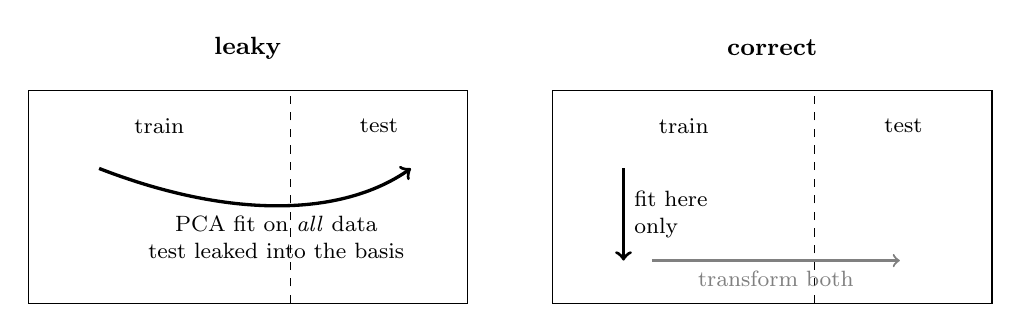
\begin{tikzpicture}[scale=0.9]
% wrong way vs right way: PCA fit scope
\node[align=center, font=\small] at (3.1,3.6) {\textbf{leaky}};
\draw (0,0) rectangle (6.2,3);
\draw[dashed] (3.7,0) -- (3.7,3);
\node[font=\footnotesize] at (1.85,2.5) {train};
\node[font=\footnotesize] at (4.95,2.5) {test};
\draw[->, very thick] (1.0,1.9) .. controls (2.8,1.2) and (4.4,1.2)
  .. (5.4,1.9) node[midway, below, font=\footnotesize, align=center]
  {PCA fit on \emph{all} data\\ test leaked into the basis};
\begin{scope}[xshift=7.4cm]
\node[align=center, font=\small] at (3.1,3.6) {\textbf{correct}};
\draw (0,0) rectangle (6.2,3);
\draw[dashed] (3.7,0) -- (3.7,3);
\node[font=\footnotesize] at (1.85,2.5) {train};
\node[font=\footnotesize] at (4.95,2.5) {test};
\draw[->, very thick] (1.0,1.9) -- (1.0,0.6)
  node[midway, right, font=\footnotesize, align=left] {fit here\\ only};
\draw[->, thick, gray] (1.4,0.6) -- (4.9,0.6)
  node[midway, below, font=\footnotesize] {transform both};
\end{scope}
\end{tikzpicture}
